\documentclass{standalone}
\usepackage{tikz}
\usetikzlibrary{patterns, positioning}
\usepackage[sfdefault]{ClearSans} %% option 'sfdefault' activates Clear Sans as the default text font
\usepackage[T1]{fontenc}

\begin{document}
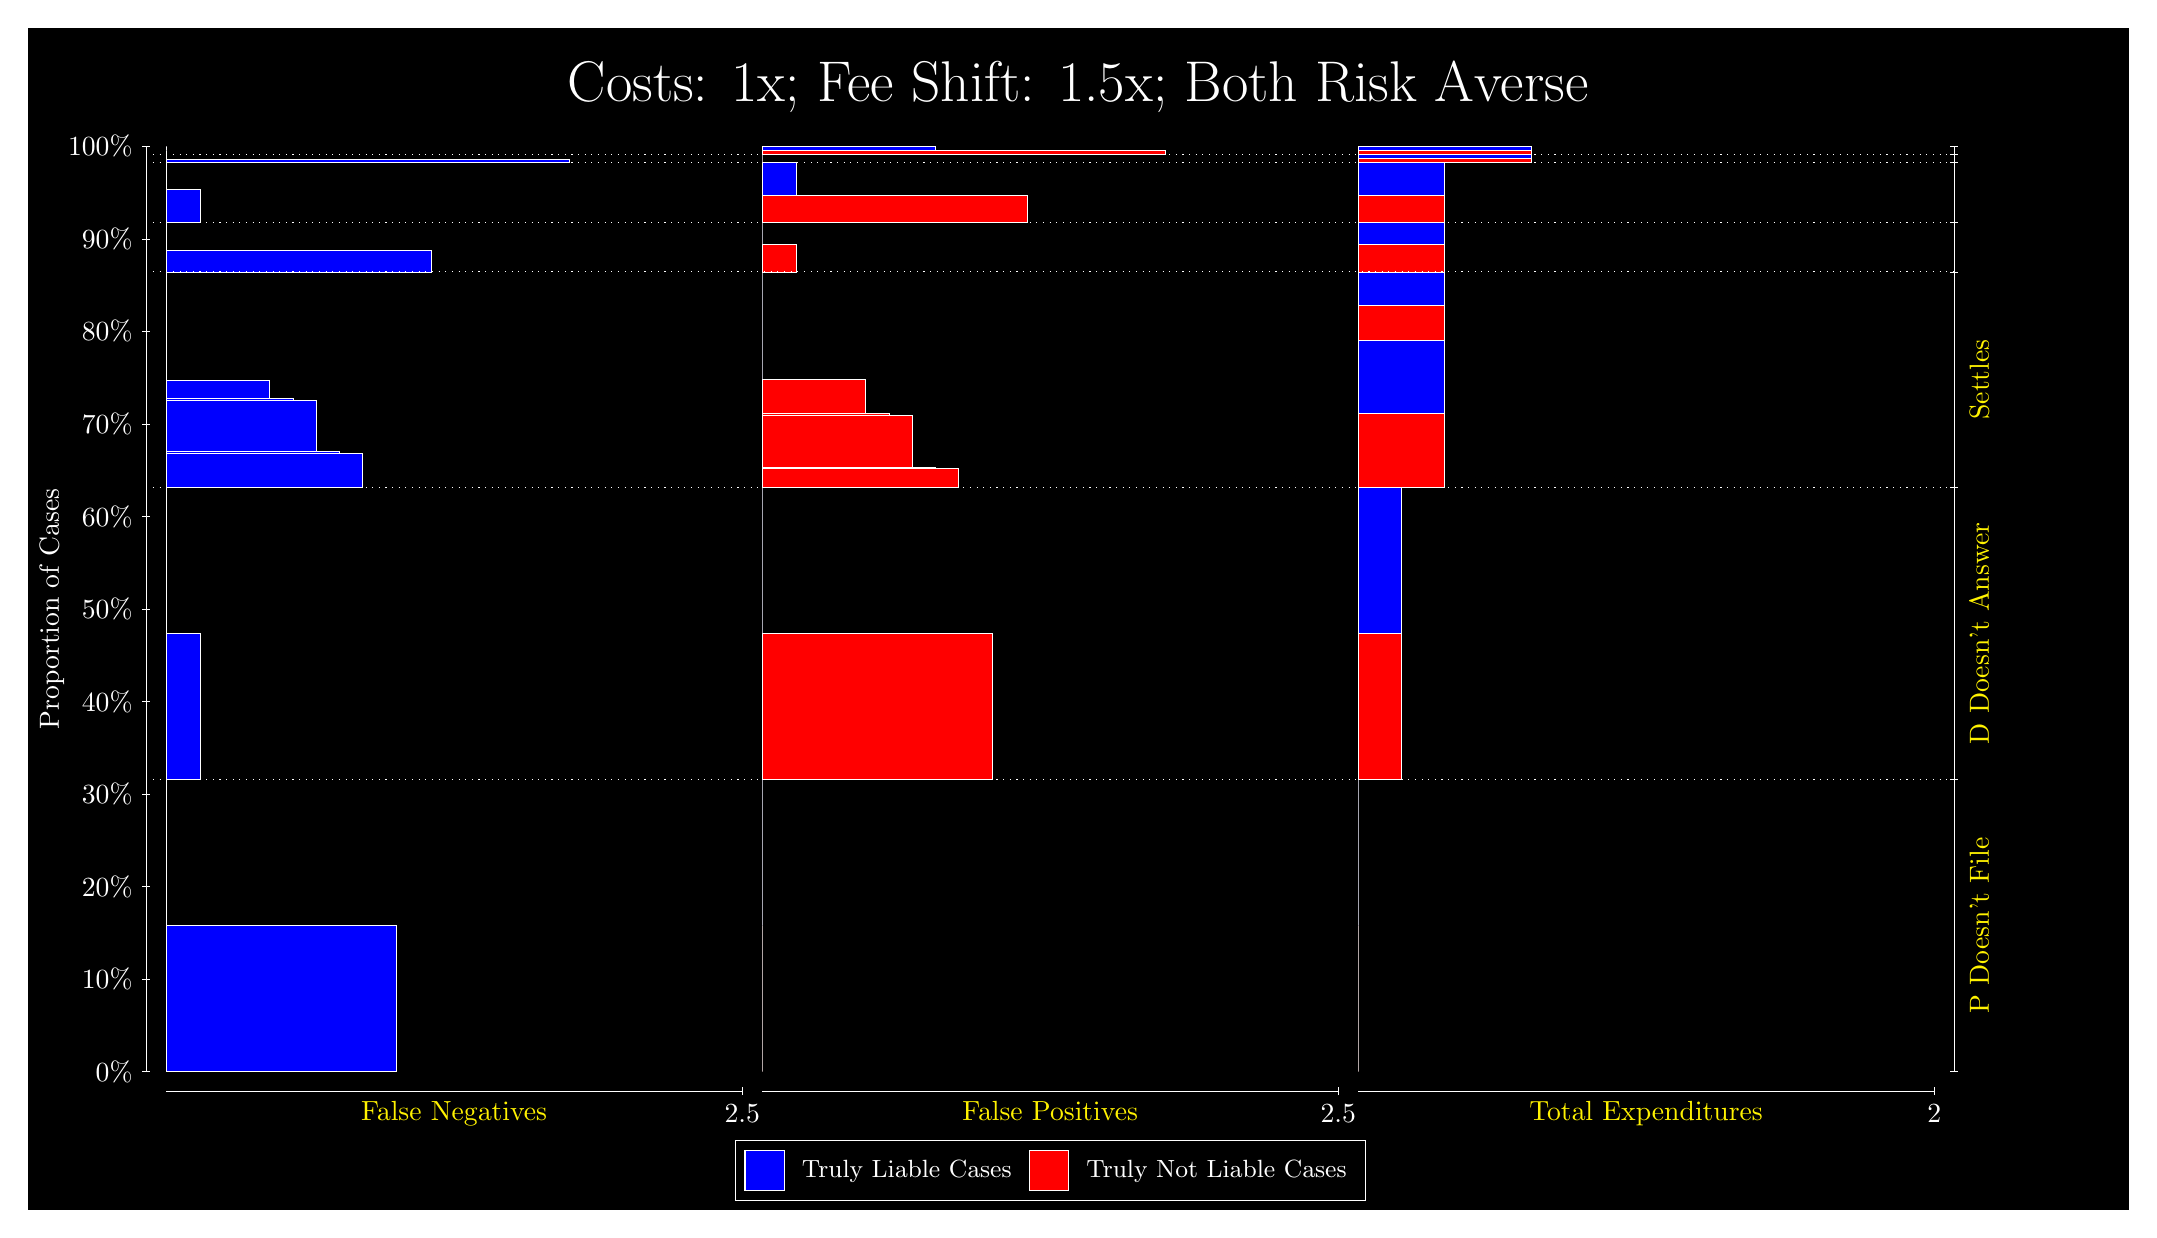
\begin{tikzpicture}
\draw[fill=black] (0,0) rectangle (26.667,15);
\draw[text=white] (0,13.5) rectangle (26.667,15) node[midway] {\huge Costs: 1x; Fee Shift: 1.5x; Both Risk Averse};
\draw[white, very thin] (1.5,1.75) -- (1.5,13.5);
\node[rotate=90, text=white, anchor=center] at (0.3, 7.625) {Proportion of Cases};
\draw[white, very thin] (1.45,1.75) -- (1.55,1.75);
\node[text=white, anchor=east] at (1.45, 1.75) {0\%};
\draw[white, very thin] (1.45,2.925) -- (1.55,2.925);
\node[text=white, anchor=east] at (1.45, 2.925) {10\%};
\draw[white, very thin] (1.45,4.1) -- (1.55,4.1);
\node[text=white, anchor=east] at (1.45, 4.1) {20\%};
\draw[white, very thin] (1.45,5.275) -- (1.55,5.275);
\node[text=white, anchor=east] at (1.45, 5.275) {30\%};
\draw[white, very thin] (1.45,6.45) -- (1.55,6.45);
\node[text=white, anchor=east] at (1.45, 6.45) {40\%};
\draw[white, very thin] (1.45,7.625) -- (1.55,7.625);
\node[text=white, anchor=east] at (1.45, 7.625) {50\%};
\draw[white, very thin] (1.45,8.8) -- (1.55,8.8);
\node[text=white, anchor=east] at (1.45, 8.8) {60\%};
\draw[white, very thin] (1.45,9.975) -- (1.55,9.975);
\node[text=white, anchor=east] at (1.45, 9.975) {70\%};
\draw[white, very thin] (1.45,11.15) -- (1.55,11.15);
\node[text=white, anchor=east] at (1.45, 11.15) {80\%};
\draw[white, very thin] (1.45,12.325) -- (1.55,12.325);
\node[text=white, anchor=east] at (1.45, 12.325) {90\%};
\draw[white, very thin] (1.45,13.5) -- (1.55,13.5);
\node[text=white, anchor=east] at (1.45, 13.5) {100\%};

\draw[white, very thin] (24.457,1.75) -- (24.457,13.5);
\draw[white, very thin] (24.407,1.75) -- (24.507,1.75);
\node[anchor=west] at (24.407, 1.75) {};
\draw[white, very thin] (24.407,5.4605) -- (24.507,5.4605);
\node[anchor=west] at (24.407, 5.4605) {};
\draw[white, very thin] (24.407,9.1711) -- (24.507,9.1711);
\node[anchor=west] at (24.407, 9.1711) {};
\draw[white, very thin] (24.407,11.905) -- (24.507,11.905);
\node[anchor=west] at (24.407, 11.905) {};
\draw[white, very thin] (24.407,12.538) -- (24.507,12.538);
\node[anchor=west] at (24.407, 12.538) {};
\draw[white, very thin] (24.407,13.294) -- (24.507,13.294);
\node[anchor=west] at (24.407, 13.294) {};
\draw[white, very thin] (24.407,13.397) -- (24.507,13.397);
\node[anchor=west] at (24.407, 13.397) {};
\draw[white, very thin] (24.407,13.5) -- (24.507,13.5);
\node[anchor=west] at (24.407, 13.5) {};

\draw[white, very thin, fill=blue] (1.75,1.75) rectangle (4.6775,3.6053);
\draw[white, very thin, fill=red] (1.75,3.6053) rectangle (1.75,5.4605);
\draw[white, very thin, fill=blue] (1.75,5.4605) rectangle (2.1891,7.3158);
\draw[white, very thin, fill=red] (1.75,7.3158) rectangle (1.75,9.1711);
\draw[white, very thin, fill=blue] (1.75,9.1711) rectangle (4.2384,9.5984);
\draw[white, very thin, fill=blue] (1.75,9.5984) rectangle (3.9457,9.6228);
\draw[white, very thin, fill=blue] (1.75,9.6228) rectangle (3.6529,10.273);
\draw[white, very thin, fill=blue] (1.75,10.273) rectangle (3.3602,10.294);
\draw[white, very thin, fill=blue] (1.75,10.294) rectangle (3.0674,10.534);
\draw[white, very thin, fill=red] (1.75,10.534) rectangle (1.75,11.905);
\draw[white, very thin, fill=blue] (1.75,11.905) rectangle (5.1167,12.184);
\draw[white, very thin, fill=red] (1.75,12.184) rectangle (1.75,12.538);
\draw[white, very thin, fill=blue] (1.75,12.538) rectangle (2.1891,12.958);
\draw[white, very thin, fill=red] (1.75,12.958) rectangle (1.75,13.294);
\draw[white, very thin, fill=blue] (1.75,13.294) rectangle (6.8732,13.341);
\draw[white, very thin, fill=red] (1.75,13.341) rectangle (1.75,13.397);
\draw[white, very thin, fill=red] (1.75,13.397) rectangle (1.75,13.445);
\draw[white, very thin, fill=blue] (1.75,13.445) rectangle (1.75,13.5);
\draw[white, very thin, fill=red] (9.3189,1.75) rectangle (9.3189,3.6053);
\draw[white, very thin, fill=blue] (9.3189,3.6053) rectangle (9.3189,5.4605);
\draw[white, very thin, fill=red] (9.3189,5.4605) rectangle (12.246,7.3158);
\draw[white, very thin, fill=blue] (9.3189,7.3158) rectangle (9.3189,9.1711);
\draw[white, very thin, fill=red] (9.3189,9.1711) rectangle (11.807,9.4052);
\draw[white, very thin, fill=red] (9.3189,9.4052) rectangle (11.515,9.4297);
\draw[white, very thin, fill=red] (9.3189,9.4297) rectangle (11.222,10.083);
\draw[white, very thin, fill=red] (9.3189,10.083) rectangle (10.929,10.104);
\draw[white, very thin, fill=red] (9.3189,10.104) rectangle (10.636,10.542);
\draw[white, very thin, fill=blue] (9.3189,10.542) rectangle (9.3189,11.905);
\draw[white, very thin, fill=red] (9.3189,11.905) rectangle (9.758,12.259);
\draw[white, very thin, fill=blue] (9.3189,12.259) rectangle (9.3189,12.538);
\draw[white, very thin, fill=red] (9.3189,12.538) rectangle (12.686,12.874);
\draw[white, very thin, fill=blue] (9.3189,12.874) rectangle (9.758,13.294);
\draw[white, very thin, fill=red] (9.3189,13.294) rectangle (9.3189,13.35);
\draw[white, very thin, fill=blue] (9.3189,13.35) rectangle (9.3189,13.397);
\draw[white, very thin, fill=red] (9.3189,13.397) rectangle (14.442,13.445);
\draw[white, very thin, fill=blue] (9.3189,13.445) rectangle (11.515,13.5);
\draw[white, very thin, fill=red] (16.888,1.75) rectangle (16.888,3.6053);
\draw[white, very thin, fill=blue] (16.888,3.6053) rectangle (16.888,5.4605);
\draw[white, very thin, fill=red] (16.888,5.4605) rectangle (17.437,7.3158);
\draw[white, very thin, fill=blue] (16.888,7.3158) rectangle (17.437,9.1711);
\draw[white, very thin, fill=red] (16.888,9.1711) rectangle (17.986,10.104);
\draw[white, very thin, fill=blue] (16.888,10.104) rectangle (17.986,11.04);
\draw[white, very thin, fill=red] (16.888,11.04) rectangle (17.986,11.477);
\draw[white, very thin, fill=blue] (16.888,11.477) rectangle (17.986,11.905);
\draw[white, very thin, fill=red] (16.888,11.905) rectangle (17.986,12.259);
\draw[white, very thin, fill=blue] (16.888,12.259) rectangle (17.986,12.538);
\draw[white, very thin, fill=red] (16.888,12.538) rectangle (17.986,12.874);
\draw[white, very thin, fill=blue] (16.888,12.874) rectangle (17.986,13.294);
\draw[white, very thin, fill=red] (16.888,13.294) rectangle (19.083,13.35);
\draw[white, very thin, fill=blue] (16.888,13.35) rectangle (19.083,13.397);
\draw[white, very thin, fill=red] (16.888,13.397) rectangle (19.083,13.445);
\draw[white, very thin, fill=blue] (16.888,13.445) rectangle (19.083,13.5);
\draw[white, dotted] (1.5,5.4605) -- (24.457,5.4605);
\draw[white, dotted] (1.5,9.1711) -- (24.457,9.1711);
\draw[white, dotted] (1.5,11.905) -- (24.457,11.905);
\draw[white, dotted] (1.5,12.538) -- (24.457,12.538);
\draw[white, dotted] (1.5,13.294) -- (24.457,13.294);
\draw[white, dotted] (1.5,13.397) -- (24.457,13.397);
\draw[white, very thin] (1.75,1.5) -- (9.0689,1.5);
\node[text=yellow, anchor=north] at (5.4094, 1.5) {False Negatives};
\draw[white, very thin] (9.0689,1.45) -- (9.0689,1.55);
\node[text=white, anchor=north] at (9.0689, 1.45) {2.5};

\draw[white, very thin] (9.3189,1.5) -- (16.638,1.5);
\node[text=yellow, anchor=north] at (12.978, 1.5) {False Positives};
\draw[white, very thin] (16.638,1.45) -- (16.638,1.55);
\node[text=white, anchor=north] at (16.638, 1.45) {2.5};

\draw[white, very thin] (16.888,1.5) -- (24.207,1.5);
\node[text=yellow, anchor=north] at (20.547, 1.5) {Total Expenditures};
\draw[white, very thin] (24.207,1.45) -- (24.207,1.55);
\node[text=white, anchor=north] at (24.207, 1.45) {2};

\node[text=yellow, centered, rotate=90] at (24.777, 3.6053) {P Doesn't File};
\node[text=yellow, centered, rotate=90] at (24.777, 7.3158) {D Doesn't Answer};
\node[text=yellow, centered, rotate=90] at (24.777, 10.538) {Settles};





\draw (12.978300999999998,1.5) node[draw=none] (baseCoordinate) {};
\begin{scope}[align=center]
        \matrix[scale=0.5, draw=white, below=0.5cm of baseCoordinate, nodes={draw}, column sep=0.1cm]{
            \node[rectangle, draw, minimum width=0.5cm, minimum height=0.5cm, fill=blue] {}; &
            \node[draw=none, font=\small, text=white] (B) {Truly Liable Cases}; &
            \node[rectangle, draw, minimum width=0.5cm, minimum height=0.5cm, fill=red] {}; &
            \node[draw=none, font=\small, text=white] (B) {Truly Not Liable Cases}; \\
            };
\end{scope}

\end{tikzpicture}
\end{document}